\documentclass[a4paper,ngerman]{scrartcl}

\usepackage{amsmath}
\usepackage{amsfonts}
\usepackage{amssymb}
\usepackage[utf8]{inputenc}
\usepackage{graphicx}
\usepackage[ngerman]{babel}
\usepackage{hyperref}
\usepackage{float}
\usepackage{caption}
\usepackage{subcaption}
\usepackage{multirow}  %for tables
\usepackage{icomma} % Handle german comma as decimal point in numbers
\usepackage{units,siunitx} % Write units with correct spacing
\usepackage{upgreek} % provide non-italic greek letters
\usepackage{url}
\usepackage{extpfeil}
%\usepackage{subfig}

% Formatting of table & figure captions
\captionsetup{font={sf,footnotesize},labelfont=bf,textfont=sl,skip=6pt}
\setlength{\abovecaptionskip}{6pt}
\setlength{\belowcaptionskip}{0pt}

\title{Black Lipid Membrane (BLM)}
\date{\today}
\author{Michel Rausch, Michael Eliachevitch}

\begin{document}

\maketitle
\tableofcontents
\newpage

\section{Einleitung}

In diesem Versuch werden Ionenkanäle in planaren Lipidmembranen untersucht. Hierbei wird der Wirkmechanismus des Antibiotikums Gramacidin A untersucht. In einer biologischen Zelle gelangen durch die entstandenen Kanäle Kationen durch die Zellmembran. Die Zelle stirbt aufgrund der Zerstörung ihres elektrochemischen Gradients [\ref{ref:mappe}].

Gramicidin beschreibt eine Gruppe Antibiotika. Dieses ist kommerziell unter Namen wie Angidin\textregistered , Mycolog\textregistered , Topsym\textregistered , Neospiron\textregistered  verfügbar. 


\section{Theoretische Grundlagen}

Die chemischen Grundlagen werden hier nicht genau behandelt. Gramicidin A1 besitzt die Summenformel $C_{99}H_{140}N_{20}O_{17}$. Es kann in der Natur von erdlebenden Bakterien beobachtet, aber auch synthetisch hergestellt werden. Mehrere Strukturen sind möglich, wobei Gramicidin A die häufigste ist. Gramicidin besitzt eine zyklische Struktur und damit einen anderen Wirkmechanismus. In diesem Experiment wird lediglich die Variante A verwendet.

\subsection{Wirkmechanismus}

Es existieren verschiedene Modelle, die Beschreiben, wie Gramicidin A in die Zellmembran integriert wird. Diese sind in Abbildung \ref{fig:wirkmechanismus} gezeigt. Auf die Einzelheiten wird nicht im Detail eingegangen.
\begin{itemize}
\item \textbf{A: Barrel Stave model} 
Hydrophobe, helixförmige Monomere bilden Poren in der Zellmembran.
\item \textbf{B: Toroidial Wormhole}  
Poremformation nahe phosphatidylethanolamine, oder phosphatidylserine Membranen. 
\item \textbf{C: Carpet model}  
Teppich-(engl. carpet-)ähnliche Anlagerung auf Membran.
\item \textbf{D} Detergent similar model
Bi- und Mizellen bilden Flächen auf der Membran. Durch deren Amphiphilie wird die Membran durchlässig.
\item \textbf{E} In-plane diffusion model
Verdünnung der Lipidschicht.
\end{itemize}

\begin{figure}
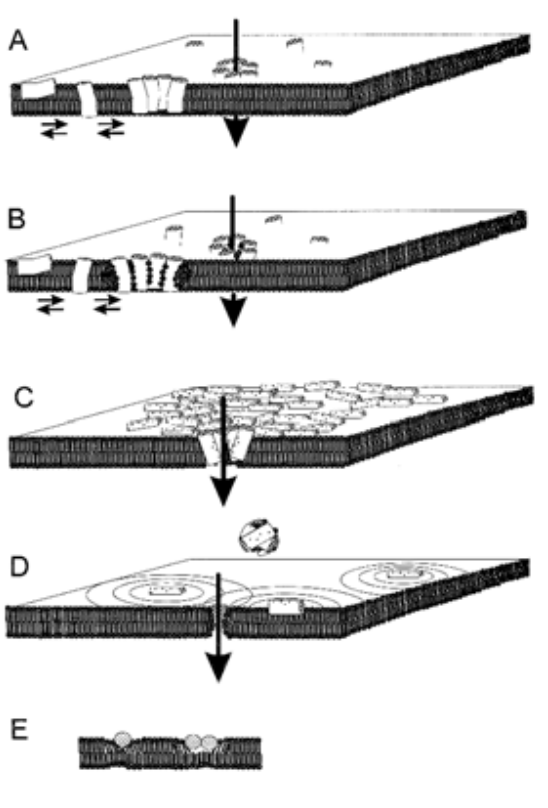
\includegraphics[width=0.5\textwidth]{abbildungen/wirkmechanismus.png}
\caption{Verschiedene Modelle zur Erklärung der Zerstörung einer Bakterienzelle mittels Peptid-Antibiotika [\ref{ref:mappe}]}
\label{fig:wirkmechanismus}
\end{figure}


\subsection{Ionentransport}

Eine Membran trennt zwei Bereiche einer wässrigen Lösung. Um sie zu überwinden, muss ein Ion eine Energie $E$ aufbringen. Die  Wahrscheinlichkeit k, eines Ions mit der Temperatur T, diese n einer Zeiteinheit zu überwinden ist der Ratenkoeffizient
\begin{equation} \label{eqn:rate}
k = k_0 e^{-\frac{E}{k_B T}},
\end{equation}
mit der Boltzmannkonstante $k_{B}$. Das Potential einer Membran lässt sich wie in Abbildung \ref{fig:potential-einfach} vorstellen. Die Ionen können in der Membran Bindungen eingehen, daher entstehen weitere Minima.

\begin{figure}
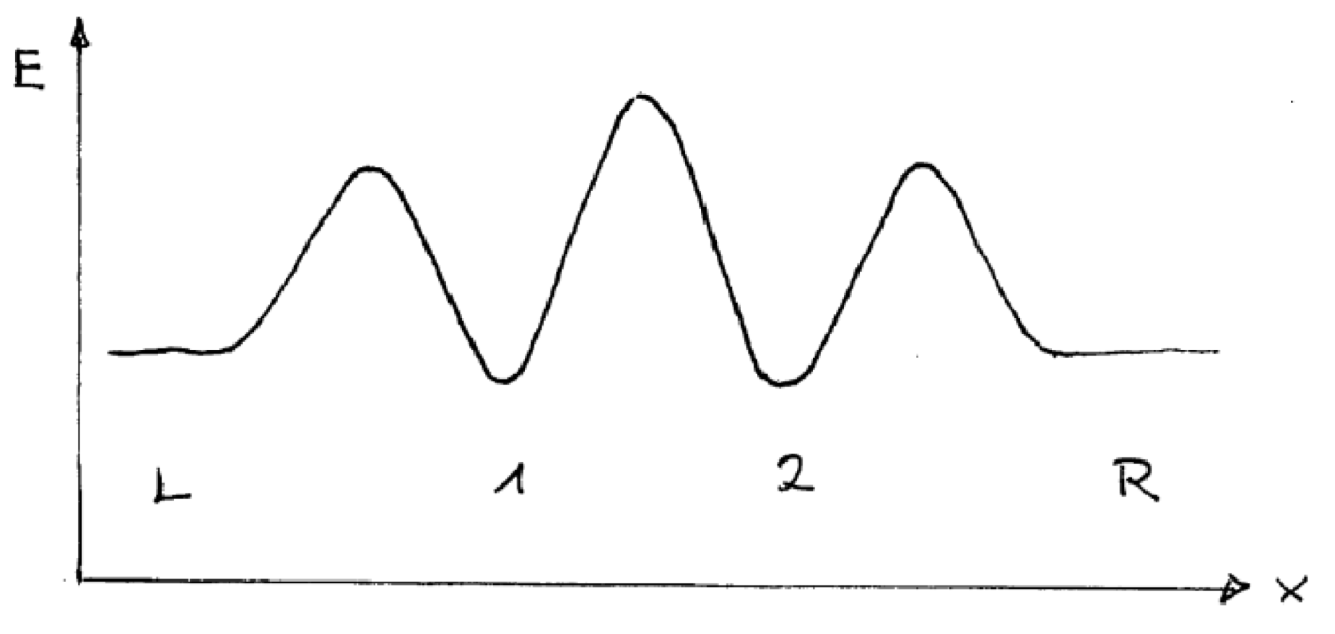
\includegraphics[width=0.6\textwidth]{abbildungen/potential-einfach.png}
\caption{Schema eines Potentials einer Pore [\ref{ref:mappe}]}
\label{fig:potential-einfach}
\end{figure}


Die Gleichung \ref{eqn:rate} wird auf den Fall des Experiments erweitert. Durch die angelegte Spannung $V_{m}$ wird das Potential asymmetrisch, wie in Abbildung \ref{fig:potential-asym} gezeigt.  Es wird die Quasistationaritätsnäherung verwendet. Die Leitfähigkeit eines einzelnen Kanals ist dann

\begin{equation}
\Lambda = \frac{k_A}{k_D} \cdot \frac{c}{k_A^{-1}+k^{-1}+k_D^{-1}} \cdot  \frac{q^2}{k_B T} .
\end{equation}

Mit der Ladung q der Ionen und den Ratenkoeffizienten $k_A$, $k_D$ und $k$ der Membran.
Hieraus ergeben sich die Zusammenhänge der makroskopisch Messbaren Größen

\begin{equation}
I_M = \lambda_M \cdot V_m
\end{equation}
und
\begin{equation}
\lambda_m = \Lambda \cdot N_p.
\end{equation}

Hierbei ist $I_M$ der gemessene Gesamtstrom an der Membran. $\lambda_M$ beschreibt die Leitfähigkeit der Membran.


\begin{figure}
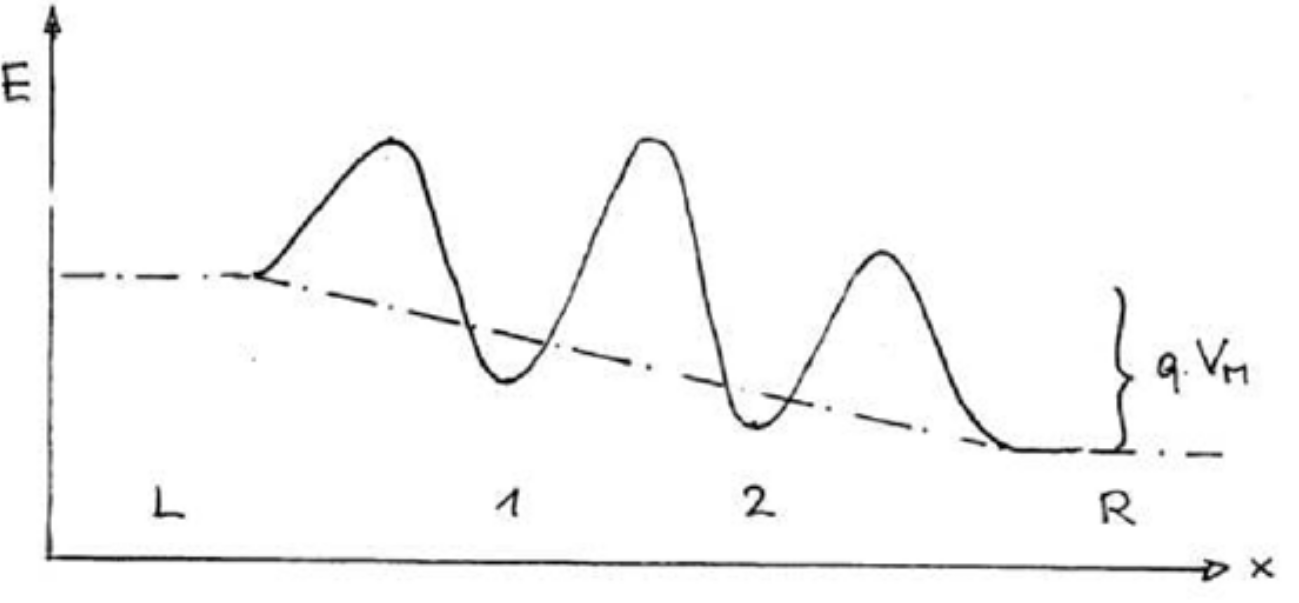
\includegraphics[width=0.6\textwidth]{abbildungen/potential-asym.png}
\caption{Schema des Potentials einer Pore mit angelegter Spannung [\ref{ref:mappe}]}
\label{fig:potential-asym}
\end{figure}



\subsubsection{Einzelkanalentstehung}

Nur Dimere des Gramicidin A führen zu einer Bildung von Ionenkanälen. Im Gleichgewicht werden Dimere gebildet und vernichtet. Dies führt zu einer variierenden Anzahl an Poren in der Membran und somit zu einer Fluktuation der Leitfähigkeit. Bei einer geringen Konzentration sind nur einzelne Kanäle vorhanden, daher ist die Quantisierung des Stromes $I_M$ deutlich erkennbar.

Die Dimerasation kann durch die Gleichung

\begin{equation}
G_1 + G_1 	\xtofrom[k_d]{k_r} G_2
\end{equation}

beschrieben werden. $k_d$ ist hier die Rate der Dissoziation und $k_r$ die der Entstehung der Dimere. Die Dissoziation folgt einem exponentiellem Zerfallsgesetz, die der Entstehungreaktion ist linear zu Konzentration. Aus dem Verlauf des Stromes über die zeit lässt sich die Zerfallsrate bestimmen.



\subsubsection{Mehrkanalentstehung}



\subsubsection{Autokorrelationsfunkion}


\subsubsection{Charakteristik einer Membran}












\clearpage
\section{Versuchsaufbau und Versuchsdurchführung}



\subsection{Versuchsaufbau und Vorbereitung der Lösungen}
\label{sec:bilayer-vorbereitung}

\begin{figure}[tb!]
  \centering
  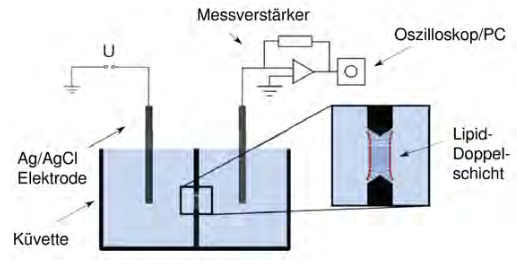
\includegraphics[width=0.8\textwidth]{abbildungen/blmaufbau.png}
  \caption{\textbf{Aufbau einer BLM ("`Black Lipid Membrane"').} \\Eine Küvette ist durch eine hydrophobe Trennwand zweigeteilt. Diese Trennwand hat ein kleines Loch in der Größenordnungen von Mikrometern, auf das eine Lipid-Doppelschicht "`aufgemalt"' wird. Da sie im getrockneten Zustand eine molekulare Dicke von nur einigen Nanometern hat, kommt es zu destruktiver Interferenz des an beiden Seiten reflektierten Lichtes und sie erscheint schwarz, weshalb die Lipid-Doppelschicht als BML bezeichnet wird. Die Küvette enthält eine Elektrolytlösung und zwischen beiden Hälften kann durch Dioden eine Gleich- oder Wechselspannung angelegt werden. Das Ablesen von elektrischen Signalen erfolgt am Oszilloskop, das hinter einen Verstärker geschaltet ist.}
  \label{fig:blmaufbau}
\end{figure}

Der typische Aufbau einer BLM ("`Black Lipid Membrane"') ist in Abbildung \ref{fig:blmaufbau} dargestellt und erklärt. \\

In unserem Fall werden als Elektrolytlösung 0.5\,M Kaliumchlorid (KCl) vorbereitet, um genügend Ionen zur Verfügung zustellen, aber auch nicht zu viele, um die Lipid-Doppelschicht nicht zu zerstören. Die Lipidlösung zum Aufmalen der BLM soll eine Konzentration von 
$\SI{3,5}{mg/ml}$ Glyzerin-Monooleat in Tetradekan haben. Zum Erzeugen der Ionenkanäle in der Membran wird das Antibiotikum Gramicidin A verwendet. Dazu wird zuerst eine
Lösung mit einer Konzentration von $\SI{0,1}{mg/ml}$ hergestellt, von der ein Teil nochmal mit Wasser verdünnt wird, um eine Konzentration von
$\SI{4}{ng/ml}$ zu erhalten. \\

Als Serienwiderstand werden $\SI{100}{k\ohm}$ verwendet und als Feedback-Widerstand $\SI{500}{k\ohm}$. Zuerst werden wir eine 
Rechteck-Wechselspannung mit einer Frequenz von 100\,Hz verwenden, die eine Amplitude zwischen 20 und 100\,mV haben soll. \\



\subsection{Erzeugung der Lidid-Doppelschicht und Messung der Membran-Kapazität}
\label{sec:capacity}
Die Küvette soll in die Apperatur eingesetzt und die Lipidlösung mit einem Teflonstäbchen auf das gereinigte Loch aufgetragen werden, wobei darauf geachtet werden sollte, dass es keine Luftblasen gibt.
Dann soll einige Minuten gewartet werden, damit die Lipid-Doppelschicht trocknet. Die Schicht wird dabei mit einer Lampe im Abstand
von 30\,cm beleuchtet. Am Anfang sollten in der Reflexion Newtonsche Ringe sichtbar sein. Wenn das nicht der Fall ist, soll mit einem
Teflonstäbchen etwas von der Schicht entfernt werden. Im getrockneten Zustand sollte die Schicht im Objektiv schwarz erscheinen, da es 
an das an der Vorder- und Rückseite der Schicht reflektierte Licht destruktiv interferiert. Außerdem sollten im getrockneten Zustand 
einer Erhöhung der Membran-Kapazität feststellbar sein. Dabei kann die Membran als Plattenkondensator angenommen werden. Die Kapazität $C$
ist dabei eine Funktion der Dicke $d$ und der Fläche $A$ der Membran
\begin{equation}
C = \epsilon_0 \epsilon_r \frac{A}{d}.
\end{equation}1

Die experimentelle Bestimmung der Kapazität erfolgt über die Messung des Relaxationszeit $\tau$ des Membranstroms $I_C$. Die Entladung erfolgt
exponentiell gemäß der Formel

\begin{equation}
  I_C(t) = - \frac{U_0}{R_C} \cdot e^{\frac{t}{\tau}} = - I_0 \cdot e^{\frac{t}{R_C C}},
\end{equation}

wobei $R_C$ den reellen Widerstand des Kondensators bezeichnet. 
Daraus folgt, dass sich die Kapazität berechnen lässt über:

\begin{equation}
  C = \frac{\tau}{R_C}.
\end{equation}

Als spezifische Kapazität pro Fläche $C_S$ soll ebenfalls bestimmt werden:

\begin{equation}
  C_S = \frac{C}{A}.
\end{equation}

Sobald die Membran trocken ist, wird in beide Hälften der Küvette die KCl Lösung eingefüllt.

\subsection{Messung einzelne Ionenkanäle}
\label{sec:singlechannels}

\subsection{Messung multipler Ionenkanäle}
\label{sec:multiplechannels}


\subsection{Noise-Analyse und Autokorrelationsfunktion}
\label{sec:noise-autocorr}

\subsection{Weitere Fragen}
\label{sec:weitere-fragen}















\section{Quellen}
\begin{enumerate}
\item Vorbereitungsmappe \label{ref:mappe}
\item pharmawiki.ch (16.11.2014) \label{ref:pharmawiki}
\end{enumerate}



\end{document}
